\documentclass[french,11pt,twoside]{VcCours}

\newenvironment{ApplicationDirecte}{\textbf{Application directe du cours :}

}{}
\newcommand{\dx}{\text{d}x}
\DeclareMathOperator{\e}{e}
\newcommand{\Sum}[2]{\ensuremath{\textstyle{\sum\limits_{#1}^{#2}}}}
\newcommand{\Int}[2]{\ensuremath{\mathchoice%
	{{\displaystyle\int_{#1}^{#2}}}
	{{\displaystyle\int_{#1}^{#2}}}
	{\int_{#1}^{#2}}
	{\int_{#1}^{#2}}
}}


\begin{document}

\Titre{PSI}{Promotion 2021--2022}{Mathématiques}{Chapitre 2 : Séries}

\tableofcontents
\separationTitre

\newpage
Dans tout le chapitre, $\mathbb{K}$ désigne $\mathbb{R}$ ou $\mathbb{C}$ et $(u_n)_{n \geq 0}$ une suite d'éléments de $\mathbb{K}$.

\section{Généralités}
\subsection{Convergence d'une série et premières propriétés}
\begin{defin}
Soit $(u_n)_{n \geq 0}$ une suite d'éléments de $\mathbb{K}$. On pose pour tout $n \in \mathbb{N}$,
$$ S_n =  u_0 + u_1 + \cdots + u_n = \sum_{k=0}^n u_k $$

\begin{itemize}
\item La suite $(S_n)_{n \geq 0}$ est appelée \textit{série} de terme général $u_n$. On la note $\dis \Sum{n \geq 0}{} u_n$, $\dis \Sum{n \in \mathbb{N}}{} u_n$ ou $\dis \Sum{}{} u_n$.
\item L'élément $S_n$ (appartenant à $\mathbb{K}$) est appelé \textit{somme partielle} d'ordre $n$ de la série.
\end{itemize}
\end{defin}

\begin{ex} \textbf{Séries géométriques.}

%
%Soit $z$ un nombre complexe. On appelle \textit{série géométrique} de raison $z$, la série $\dis \Sum{n \geq 0}{} z^n$. 
%
%Pour tout $n \in \mathbb{N}$, on a :
%$$ S_n = \sum_{k=0}^n z^k = \left\lbrace \begin{array}{cl}
%\dis \frac{1-z^{n+1}}{1-z} & \hbox{ si }  z \neq 1 \\[0.3cm]
%n + 1 & \hbox{ sinon} \\
%\end{array}\right.$$

\vspace{5cm}
\end{ex}

\begin{rems}
\item Si une suite a pour premier indice $n_0 \in \mathbb{N}$, la série de terme général $u_n$ a aussi pour premier indice $n_0$ et on note cette série $\dis \Sum{n \geq n_0}{} u_n$. Ainsi les sommes partielles $S_n$ ne sont définies que pour $n \geq n_0$. 

\medskip

Dans la suite du chapitre, on considérera dans les résultats uniquement le cas où $n_0=0$ (les résultats s'adaptent facilement).
\item On associe à toute suite une série. Réciproquement, toute suite peut être vue comme une série :

%
%fixons une suite $(S_n)_{n \geq 0}$ d'éléments de $\mathbb{K}$. En posant $u_0=S_0$ et pour tout $n \in \mathbb{N}^*$, $u_n = S_n - S_{n -1}$, on a :
%$$ \forall n \in \mathbb{N}, \quad \sum_{k=0}^n u_k = S_n$$
%par télescopage. Ainsi toute suite peut être vue comme une série.

\vspace{4cm}
\end{rems}

\begin{defin}
La série de terme général $u_n$ est dite \textit{convergente} si la suite des sommes partielles $(S_n)_{n \geq 0}$ est convergente. Autrement dit, si il existe $S \in \mathbb{K}$ tel que :
$$ \lim_{n \rightarrow + \infty} \sum_{k=0}^n u_k = S $$
En cas de convergence, la limite $S$ est notée $\Sum{k=0}{+ \infty} u_k$ et est appelée \textit{somme} de la série.
\end{defin}

\begin{defin} Si une série ne converge pas, on dit qu'elle est \textit{divergente}.
\end{defin}

\begin{rems}
\item La somme d'une série (quand elle existe) est unique (par unicité de la limite de la suite des sommes partielles).
\item Déterminer la \textit{nature} d'une série revient à étudier la convergence ou la divergence de celle-ci.
\end{rems}

\begin{exa} Donner les sommes partielles de $\dis \Sum{n \geq 0}{} n^3$ et préciser la nature de cette série.
\end{exa} 

\textbf{Extrait du rapport de Mines-Pont 2003.} \og De trop nombreux étudiants confondent la notion de série et la somme d'une telle série quand elle converge.  Plus généralement, on déplore un amalgame entre les notations : $\Sum{}{} u_n, \,  \Sum{n \geq 0}{} u_n,  \, \Sum{k = 0}{n} u_k$ et $\Sum{k =0}{+ \infty} u_k$ \fg 

\medskip


\begin{thm} Si une série de terme général $u_n$ converge alors $(u_n)_{n \geq 0}$ converge vers $0$. La réciproque est fausse. \end{thm}

\begin{preuve} 

\vspace{4cm}
%En notant $(S_n)_{n \geq 0}$ la suite des sommes partielles de cette série, on a pour tout entier $n \geq 1$ :
%$$ u_n = S_{n}-S_{n-1}$$
%Et ainsi, si $(S_n)_{n \geq 0}$ converge vers $S$, $(u_n)_{n \geq 0}$ converge vers $S-S=0$.
%
%\bigskip
%
%Montrons maintenant que la série harmonique diverge. Pour tout $n \in \mathbb{N}^*$, on pose :
%$$ H_n = \sum_{k=1}^n \frac{1}{k}$$
%On a pour tout $n \in \mathbb{N}^*$ :
%\begin{equation}\label{Harmonique}
%H_{2n}-H_n =  \sum_{k=1}^{2n} \frac{1}{k} -  \sum_{k=1}^n \frac{1}{k} =  \sum_{k=n+1}^{2n} \frac{1}{k}
%\end{equation}
%Or si $k \in \Interv{n+1}{2n}$, on a par décroissance de la fonction inverse sur $\mathbb{R}_+^{*}$ :
%$$ \frac{1}{2n} \leq \frac{1}{k} \leq \frac{1}{n+1} $$
%et ainsi par (\ref{Harmonique}), on a :
%\begin{equation}\label{Harmonique2} H_{2n}-H_n \geq  \sum_{k=n+1}^{2n} \frac{1}{2n} = (2n-(n+1)+1) \frac{1}{2n} = \frac{1}{2}
%\end{equation}
\end{preuve}

\begin{exa} Montrer que $\Sum{n\geq 1}{} \ln \left(1 + \frac{1}{n} \right)$ diverge (\textit{cela fournit une série divergente dont le terme général tend vers $0$}).
\end{exa}


\begin{att} Le résultat précédent est uniquement une condition nécessaire de convergence ! Autrement dit, si le terme général d'une série converge vers $0$, on ne peut rien conclure pour la convergence de cette série. 
\end{att}

\begin{cor}
Si le terme général d'une série ne converge pas vers $0$, la série est divergente. On dit qu'elle est \textit{grossièrement divergente}.
\end{cor}

%\begin{ex} Reprenons l'exemple de la série géométrique de raison $z$. Distinguons trois cas :
%
%\begin{itemize}
%\item Si $\vert z \vert < 1$, $(z^{n+1})_{n \geq 0}$ converge vers $0$ et ainsi $\Sum{n\geq 0}{} z^n$ converge et sa somme est égale à :
%$$ \sum_{k=0}^{+ \infty} z^k = \frac{1}{1-z}$$
%\item Si $z=1$, $\dis \lim_{n \rightarrow + \infty} S_n = \lim_{n \rightarrow + \infty} n+1 = +\infty $ donc la série diverge.
%\item Si $\vert z \vert \geq 1$ avec $z \neq 1$ alors $(z^{n+1})_{n \geq 0}$ diverge et il en est alors de même de la suite des sommes partielles. Dans ce cas, la série diverge.
%\end{itemize}
%\end{ex}

\begin{defip}
Soit $\Sum{n\geq 0}{} u_n$ une série.
\begin{itemize}
\item Pour tout $m \in \mathbb{N}$, $\Sum{n\geq 0}{}u_n$ et $\Sum{n\geq m+1}{}u_n$ sont de même nature.
\item En cas de convergence, la somme de $\Sum{n\geq m+1}{}u_n$, que l'on note :
$$ R_m = \sum_{k= m+1}^{+\infty}u_k$$
est appelé \textit{reste} d'ordre d'ordre $m$ de la série. 
\item La suite $(R_m)_{m \geq 0}$ converge vers $0$.
\end{itemize}
\end{defip}
%
\begin{preuve}

\vspace{6cm}
%Pour tout $n \geq m+1$, on a par la relation de Chasles :
%\begin{equation}\label{reste}
%\sum_{k=0}^{n} u_k = \sum_{k=0}^{m} u_k + \sum_{k=m+1}^{n} u_k
%\end{equation}
%Ainsi les sommes partielles des séries $\Sum{n\geq 0}{}u_n$ et $\Sum{n\geq m+1}{}u_n$ ne différent que de la constante $\Sum{k=0}{m} u_k$ et sont donc de même nature.
%
%En cas de convergence, en passant à la limite quand $n$ tend vers $+ \infty$ dans (\ref{reste}), on a :
%$$ \sum_{k=0}^{+ \infty} u_k = \sum_{k=0}^{m} u_k + R_m$$
%et donc :
%$$ R_m = \sum_{k=0}^{+ \infty} u_k - \sum_{k=0}^{m} u_k$$
%On a alors :
%$$ \lim_{n \rightarrow + \infty} R_m = \sum_{k=0}^{+ \infty} u_k - \sum_{k=0}^{+ \infty} u_k = 0$$
\end{preuve}
%
%\begin{ex} Si $\vert z \vert <1$, le reste d'ordre $m$ de la série géométrique de raison $z$ vaut :
%$$R_m  = \sum_{k = m+1}^{+ \infty} z^k = \sum_{k = 0}^{+ \infty} z^k - \sum_{k = 0}^{m} z^k = \dfrac{1}{1-z} - \dfrac{1-z^{m+1}}{1 - z} = \dfrac{z^{m+1}}{1-z} $$
%\end{ex}

%Les séries géométriques interviennent de manière important dans plusieurs chapitres. Le Théorème suivant (prouvé en plusieurs parties ci-dessus) est donc crucial : 


\subsection{Quelques exemples}
\subsubsection{Séries géométriques}

\begin{thm} 
Soit $z \in \mathbb{C}$. La série géométrique $\dis \Sum{n \geq 0}{} z^n$ converge si et seulement si $\vert z \vert <1$. On a dans ce cas : 
$$ \sum_{k=0}^{+ \infty} z^k = \phantom{\frac{1}{1-z}}$$
Les expressions des restes sont données pour tout $m \in \mathbb{N}$ par :
$$ \sum_{k=m+1}^{+ \infty} z^k = \phantom{\frac{z^{m+1}}{1-z}}$$
\end{thm}

\begin{preuve}  
%Soit $z$ un nombre complexe. On sait que pour tout $n \in \mathbb{N}$, on a :
%$$ S_n = \sum_{k=0}^n z^k = \left\lbrace \begin{array}{cl}
%\dis \frac{1-z^{n+1}}{1-z} & \hbox{ si }  z \neq 1 \\[0.3cm]
%n + 1 & \hbox{ sinon} \\
%\end{array}\right.$$
%\begin{itemize}
%\item Si $\vert z \vert < 1$, $(z^{n+1})_{n \geq 0}$ converge vers $0$ et ainsi $\Sum{n\geq 0}{} z^n$ converge et sa somme est égale à :
%$$ \sum_{k=0}^{+ \infty} z^k = \frac{1}{1-z}$$
%\item Si $\vert z \vert \geq 1$ alors la série diverge grossièrement.
%\end{itemize}
%Si $\vert z \vert <1$, le reste d'ordre $m$ de la série géométrique de raison $z$ vaut :
%$$R_m  = \sum_{k = m+1}^{+ \infty} z^k = \sum_{k = 0}^{+ \infty} z^k - \sum_{k = 0}^{m} z^k = \dfrac{1}{1-z} - \dfrac{1-z^{m+1}}{1 - z} = \dfrac{z^{m+1}}{1-z} $$

\vspace{9cm}
\end{preuve}

\subsubsection{Série harmonique}

On appelle \textit{série harmonique} la série $\dis \Sum{n \geq 1}{} \dfrac{1}{n} \cdot$

\begin{thm} La série harmonique diverge.
\end{thm}

\begin{preuve} Voir application directe du cours 3 du chapitre 1.
%
%\vspace{4cm}
%Raisonnons par l'absurde : si la série harmonique converge, la suite $(H_n)_{n \geq 1}$ est convergente donc la suite extraite de celle-ci $(H_{2n})_{n \geq 1}$ est aussi convergente et de même limite. Ainsi :
%$$ \lim_{n \rightarrow + \infty} H_{2n}-H_n = 0$$
%Mais d'après (\ref{Harmonique2}), la suite $(H_{2n}-H_n)_{n \geq 1}$ est minorée par $\dfrac{1}{2}$ et ne peut donc pas converger vers $0$. On obtient ainsi une absurdité et ainsi la série harmonique diverge.
\end{preuve}

\begin{rem} La série harmonique diverge grossièrement.
\end{rem}

\subsubsection{Série harmonique alternée}

On appelle \textit{série harmonique alternée} la série $ \Sum{n \geq 1}{} \dfrac{(-1)^{n-1}}{n} \cdot$

\medskip

Notons $(S_n)_{n \geq 1}$ les sommes partielles de cette série.
% on a pour tout entier $n \geq 1$,
%\begin{align*}
%S_n & = \Sum{k=1}{n} \dfrac{(-1)^{k-1}}{k} \\
%%& = \Sum{k=1}{n} (-1)^{k-1} \Int{0}{1} x^{k-1}  \, \dx\\
%& =   \Int{0}{1} \Sum{k=1}{n} (-x)^{k-1} \dx \\
%\end{align*}
%par linéarité de l'intégrale. Par somme des termes d'une suite géométrique (en remarquant que si $x \in [0,1]$, $-x \neq 1$) :
%\begin{align*}
%S_n & = \Int{0}{1} \frac{1-(-x)^{n}}{1+x} \dx \\
%& = \Int{0}{1} \frac{1}{1+x} \dx - \Int{0}{1} \frac{(-x)^{n}}{1+x} \dx \qquad \hbox{(linéarité de l'intégrale)}\\
%& = \left[ \ln(1+x) \right]_0^1 - \Int{0}{1} \frac{(-x)^{n}}{1+x} \dx \\
%& = \ln(2) - (-1)^n\Int{0}{1} \frac{x^{n}}{1+x} \dx \\
%\end{align*}
%Remarquons maintenant que pour tout $x \in [0,1]$, $1 \leq 1+x \leq 2$ et donc par décroissance de la fonction inverse sur $\mathbb{R}_+^{*}$,
%$$ \frac{1}{2} \leq \frac{1}{1+x} \leq 1$$
%puis sachant que $x^n \geq 0$,
%$$ 0 \leq  \frac{x^n}{1+x} \leq x^n$$
%Par croissance de l'intégrale ($0 \leq 1$), on obtient alors :
%$$ 0 \leq \int_{0}^{1} \frac{x^{n+1}}{1+x} \dx \leq \int_{0}^{1} x^{n+1} \dx = \frac{1}{n+1}$$
%Par théorème d'encadrement, la suite de terme général $\Int{0}{1} \frac{x^{n+1}}{1+x} \dx$ converge donc vers $0$ et par produit avec une suite bornée, il en est de même pour la suite de terme général $(-1)^n\Int{0}{1} \frac{x^{n+1}}{1+x} \dx$. Ainsi $(S_n)_{n \geq 1}$ converge et l'on a :
%$$ \lim_{n \rightarrow + \infty} S_n = \lim_{n \rightarrow + \infty} \ln(2) - (-1)^n \Int{0}{1} \frac{x^{n}}{1+x} \dx = \ln(2)$$
%Ainsi, la série harmonique alternée converge et somme est $\ln(2)$.

\newpage

\subsubsection{Séries télescopiques}

On appelle \textit{série télescopique} toute série de la forme $\Sum{n\geq 0}{} a_{n+1}-a_n$ où $(a_n)_{n \geq 0}$ est une suite d'éléments de $\mathbb{K}$.

\begin{prop}
La série télescopique $\Sum{n\geq 0}{} a_{n+1}-a_n$ converge si et seulement si la suite $(a_n)_{n \geq 0}$ converge.
\end{prop}

\begin{preuve} 
\vspace{3cm}
%Pour tout $n \in \mathbb{N}$, on a :
%$$ \sum_{k=0}^{n} a_{k+1}-a_k = a_{n+1}-a_0$$
%par télescopage et le résultat est alors évident.
\end{preuve}

\medskip

\begin{exa} Étudier la nature de $\dis \Sum{n\geq 1}{} \dfrac{1}{n(n+1)}$ et donner la somme en cas de convergence.

%
%Pour tout $n \in \mathbb{N}$, on a :
%$$ \sum_{k=1}^{n} \frac{1}{k(k+1)} =   \sum_{k=1}^{n} \frac{1+k-k}{k(k+1)} =   \sum_{k=1}^{n} \frac{1}{k} - \frac{1}{k+1} = 1- \frac{1}{n+1}$$
%par télescopage. On a donc :
%$$ \lim_{n \rightarrow + \infty} 1- \frac{1}{n+1} = 1$$
%La série $\dis \Sum{n\geq 1}{} \dfrac{1}{n(n+1)}$ est donc convergente et $\dis \Sum{k=1}{+\infty} \dfrac{1}{k(k+1)}  = 1.$
\end{exa}


\section{Quelques propriétés}

On munit l'ensemble des séries numériques d'une loi de composition interne $+$ et d'une loi de composition externe $\cdot$ de la manière suivante : pour toutes séries $\Sum{n \geq 0}{} u_n$ et $\Sum{n \geq 0}{} v_n$ et tout scalaire $\lambda \in \mathbb{K}$, on pose :
\begin{align*}
\Sum{n \geq 0}{} u_n + \Sum{n \geq 0}{} v_n  & = \Sum{n \geq 0}{} u_n+v_n \\
\lambda \cdot \Sum{n \geq 0}{} u_n & = \Sum{n \geq 0}{} \lambda u_n
\end{align*}



\begin{prop}
L'ensemble des séries convergentes est un $\mathbb{K}$-espace vectoriel.

Autrement dit, si $\Sum{n \geq 0}{} u_n$ et $\Sum{n \geq 0}{} v_n$ sont deux séries convergentes et si $\lambda \in \mathbb{R}$ alors la série $\Sum{n \geq 0}{} (\lambda u_n +v_n)$ est convergente. On a de plus : 
$$ \sum_{k=0}^{+ \infty} (\lambda u_k + v_k) = \lambda  \sum_{k=0}^{+ \infty}  u_k +  \sum_{k=0}^{+ \infty}  v_k$$
\end{prop}

\begin{preuve}
Il suffit d'utiliser la linéarité de la somme (finie) et le fait que l'ensemble des suites convergentes est un $\mathbb{K}$-espace vectoriel.
\end{preuve}

\begin{rem} La somme de deux séries convergentes est donc convergente. Il faut faire attention à ne pas dire n'importe quoi dans les autres cas :
\begin{itemize}
\item La somme d'une série convergente et d'une série divergente est divergente (sinon la série divergente s'écrirait comme la différence de deux séries convergentes donc serait convergente).
\item La somme de deux séries divergentes peut être divergente (somme de la série harmonique avec elle-même) ou convergente :  $\Sum{n \geq 0}{} - 1 +  \Sum{n \geq 0}{} 1 = \Sum{n \geq 0}{} 0.$
\end{itemize}
\end{rem}

\begin{prop} Si deux suites ont les mêmes termes à partir d'un certain rang, les séries associées sont de même nature.
\end{prop}

\begin{preuve}
A partir d'un certain rang, les sommes partielles ne différeront qu'une d'une constante fixe.
\end{preuve}

\begin{prop}\label{ConvSerCompl}
Soit $(u_n)_{n \geq 0}$ une suite complexe. Les assertions suivantes sont équivalentes :

\begin{enumerate}
\item $\Sum{n \geq 0}{} u_n$ converge.
\item $\Sum{n \geq 0}{} \Re e(u_n)$ et $\Sum{n \geq 0}{} \Im m(u_n)$ convergent.
\end{enumerate}
Si l'une des deux assertions précédentes est vérifiée, on a alors :
$$ \sum_{k=0}^{+ \infty} u_k = \sum_{k=0}^{+ \infty} \Re e(u_k) + i \sum_{k=0}^{+ \infty} \Im m(u_k)$$
\end{prop}

\begin{preuve} 
Cela provient du fait qu'une suite complexe est convergente si et seulement si sa partie réelle et sa partie imaginaire convergent.
\end{preuve}

\begin{ex} Montrons que $\Sum{n \geq 0}{} \dfrac{\cos(n \pi/3)}{2^n}$ converge et donnons sa somme.

\vspace{9.5cm}
\end{ex}

\section{Comparaison série-intégrale}

Donnons le principe :

%
%Dans cette section, nous étudions une méthode cruciale pour l'étude des séries : la comparaison série-intégrale. Il est important de savoir retrouver le raisonnement rapidement (il suffit de s'aider d'un bon dessin).
%
%Soit $f$ une fonction continue et décroissante sur $[n_0, + \infty[$ où $n_0 \in \mathbb{N}$. Fixons $k \in \mathbb{N}$ supérieur ou égal à $n_0$. Par décroissance de $f$ sur $[k,k+1]$, on a pour tout $x \in [k,k+1]$,
%$$ f(k+1) \leq f(x) \leq f(k)$$
%La fonction $f$ est continue sur $[k,k+1]$ donc par croissance de l'intégrale :
%$$ \int_{k}^{k+1} f(k+1) \dx \leq \int_{k}^{k+1} f(x) \dx \leq \int_{k}^{k+1} f(k) \dx$$
%ou encore 
%\begin{equation}\label{SerieInt} f(k+1) \leq  \int_{k}^{k+1} f(x) \dx \leq  f(k) 
%\end{equation}
%On retrouve cette inégalité sur le graphique suivant :
%
%\vspace{0.3cm}
%
%\begin{center}
%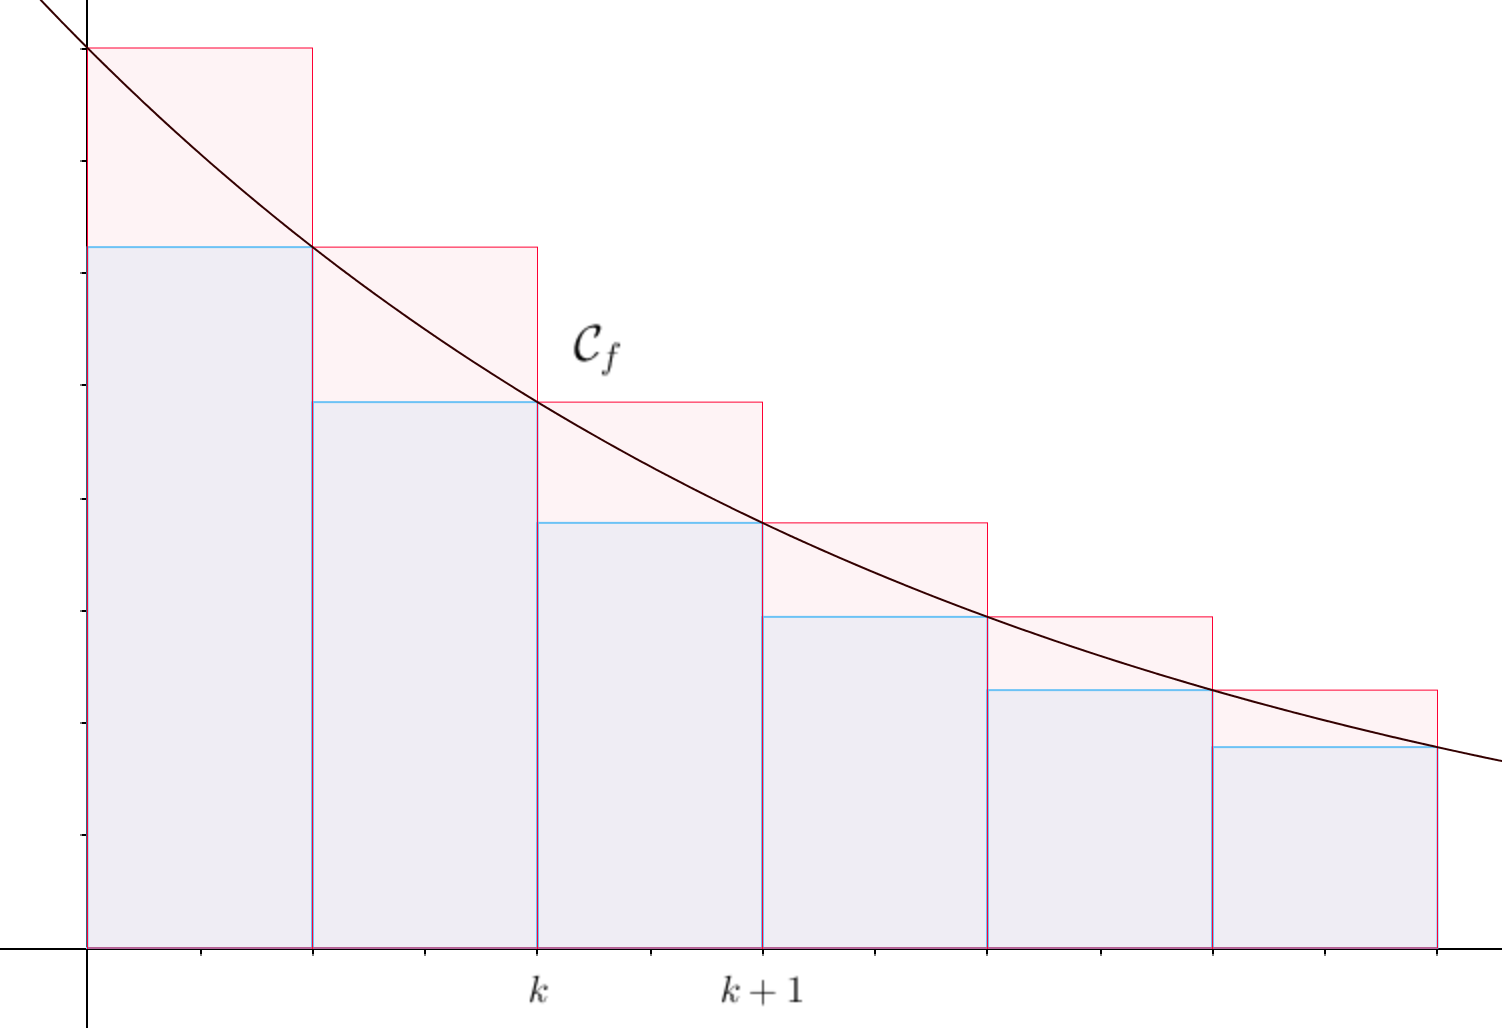
\includegraphics[scale=0.3]{serieInt}
%\end{center}
%
%Soit $n \in \mathbb{N}$. En sommant l'inégalité de gauche de (\ref{SerieInt}) de $n_0$ à $n-1$ et l'inégalité de droite de $n_0$ à $n$, on obtient :
%$$ \sum_{k=n_0}^{n-1} f(k+1) \leq  \sum_{k=n_0}^{n-1} \int_{k}^{k+1} f(x) \dx \quad \hbox{ et } \quad \sum_{k=n_0}^{n} \int_{k}^{k+1} f(x) \dx \leq \sum_{k=n_0}^n f(k) $$
%et donc par la relation de Chasles :
%$$ \sum_{k=n_0}^{n-1} f(k+1) \leq  \int_{n_0}^{n} f(x) \dx \quad \hbox{ et } \quad \int_{n_0}^{n+1} f(x) \dx \leq \sum_{k=n_0}^n f(k)$$
%ou encore :
%$$ \sum_{k=n_0}^n f(k) - f(n_0)  \leq  \int_{n_0}^{n} f(x) \dx \quad \hbox{ et } \quad \int_{n_0}^{n+1} f(x) \dx \leq \sum_{k=n_0}^n f(k)$$
%Cela permet d'obtenir un encadrement de la somme partielle de la série terme général $f(n)$ :
%$$\int_{n_0}^{n+1} f(x) \dx \leq \sum_{k=n_0}^n f(k) \leq \int_{n_0}^{n} f(x) \dx +f(n_0)$$
%
%\vspace{0.3cm}

\newpage

\textbf{Application : la série harmonique.} 

%En appliquant le procédé précédent à la fonction inverse sur $[1, + \infty[$ (qui vérifie les hypothèses souhaitées), on obtient que pour tout $n \in \mathbb{N}^*$,
%$$\int_{1}^{n+1} \frac{1}{x} \dx \leq \sum_{k=1}^n \frac{1}{k} \leq \int_{1}^{n} \frac{1}{x} \dx +1$$
%et ainsi :
%$$ \ln(n+1) \leq \sum_{k=1}^n \frac{1}{k} \leq \ln(n) +1$$
%Par Théorème d'encadrement, on prouve la divergence des sommes partielles vers $+ \infty$ et on retrouve ainsi la divergence de la série harmonique. On peut en faire faire mieux : pour tout entier $n \geq 2$, on a :
%\begin{equation}\label{Serihar}
% \frac{\ln(n+1)}{\ln(n)} \leq \frac{1}{\ln(n)} \sum_{k=1}^n \frac{1}{k} \leq 1 + \frac{1}{\ln(n)}
% \end{equation}
% 
%Or $\ln(n+1) \underset{+ \infty}{\sim} \ln(n)$ (on a $\ln(n+1) = \ln(n) + \ln \left(1+ \frac{1}{n}\right)$ et $\ln \left(1+ \frac{1}{n}\right) = o(1)$) et $1 + \frac{1}{\ln(n)}$ tend vers $1$ quand $n$ tend vers $\infty$. Par Théorème d'encadrement, on a alors par (\ref{Serihar}) :
%$$ \sum_{k=1}^n \frac{1}{k} \underset{+ \infty}{\sim} \ln(n)$$

\vspace{14.5cm}

%\newpage
%
%$\phantom{test}$
%\vspace{5cm}

\begin{retenir} Une comparaison série-intégrale peut permettre d'étudier la nature d'une série et d'obtenir un équivalent des sommes partielles.
\end{retenir}
%
%\medskip
%
%\textbf{Application 2 : trouver un équivalent de $\Sum{k = 2}{n} \dfrac{\ln(k)}{k}$ quand $n$ tend vers $+\infty$.}
%
%\vspace{10cm}
%La fonction $x \mapsto \frac{\ln(x)}{x}$ est décroissante (simple étude de fonction) et continue sur $[2, + \infty[$. Par comparaison série-intégrale, on a pour tout $n \geq 2$,
%$$ \int_{2}^{n+1} \frac{\ln(x)}{x} \dx \leq \sum_{k=2}^n \frac{\ln(k)}{k} \leq \int_{2}^{n} \frac{\ln(x)}{x} \dx +\frac{\ln(2)}{2}$$
%et ainsi :
%$$ \left[ \frac{\ln(x)^2}{2} \right]_2^{n+1} \leq \sum_{k=2}^n \frac{\ln(k)}{k} \leq \left[ \frac{\ln(x)^2}{2} \right]_2^{n} +\frac{\ln(2)}{2}$$
%Et finalement :
%$$ \frac{\ln(n+1)^2}{2} - \frac{\ln(2)^2}{2} \leq \sum_{k=2}^n \frac{\ln(k)}{k} \leq\frac{\ln(n)^2}{2} - \frac{\ln(2)^2}{2} + \frac{\ln(2)}{2}$$
%En utilisant que $\ln(n+1) \underset{+ \infty}{\sim} \ln(n)$ donc $\ln(n+1)^2 \underset{+ \infty}{\sim} \ln(n)^2$ (par produit) et en divisant l'inégalité précédente par $\dfrac{\ln(n)^2}{2}$, on obtient par Théorème d'encadrement que :
%$$  \sum_{k=1}^n \frac{\ln(k)}{k} \underset{+ \infty}{\sim} \frac{\ln(n)^2}{2}$$

\begin{exa} Étudier la nature de $\dis \Sum{n \geq 2}{}  \dfrac{1}{n\ln(n)}$ à l'aide d'une comparaison série-intégrale.
\end{exa}
\section{Séries à termes positifs}
\subsection{Critères de comparaison}
\begin{prop}\label{SATP} Soit $\Sum{n \geq 0}{} u_n$ une série à \textit{termes positifs}. Alors :
\begin{enumerate}
\item La suite des sommes partielles est croissante.
\item La série est convergente si et seulement si la suite des sommes partielles est majorée.
\end{enumerate}
\end{prop}


\begin{preuve}
%En notant $(S_n)_{n \geq 0}$ la suite des sommes partielles, on a pour tout $n \geq 0$,
%$$ S_{n+1}-S_n = u_{n+1} \geq 0$$
%Ainsi $(S_n)_{n \geq 0}$ est une suite croissante et converge si et seulement si elle est majorée (d'après le Théorème de la limite monotone).

\vspace{3cm}
\end{preuve}

\begin{rem} Si la suite des sommes partielles n'est pas majorée, elle tend donc vers $+ \infty$. Ainsi, une série à termes positifs divergente a nécessairement une suite des sommes partielles divergente vers $+ \infty$.
\end{rem}

\begin{thm}[CCSATP]
Soient $(u_n)_{n \geq 0}$ et $(v_n)_{n \geq 0}$ deux suites à \textit{termes positifs}.

\begin{enumerate}
\item Supposons que pour tout $n \in \mathbb{N}$, $u_n \leq v_n$. Alors :

\begin{itemize}
\item La convergence de $\Sum{n \geq 0}{} v_n$ implique la convergence de $\Sum{n \geq 0}{} u_n$ et on a dans ce cas :
$$ \sum_{k=0}^{ + \infty} u_k \leq  \sum_{k=0}^{+ \infty} v_k $$
\item  La divergence de $\Sum{n \geq 0}{} u_n$ implique la divergence de $\Sum{n \geq 0}{} v_n$.
\end{itemize}
\item Si $u_n \underset{+\infty}{\sim} v_n$ alors \phantom{les séries $\Sum{n \geq 0}{} u_n$ et $\Sum{n \geq 0}{} v_n$ sont de même nature.}
\end{enumerate}
\end{thm}

\begin{rem} Le résultat lié à l'équivalence reste vrai pour des séries à termes généraux négatifs. De plus, si les termes généraux sont équivalents, la positivité (ou la négativité) d'un des termes généraux implique la positivité (ou la négativité) de l'autre (à partir d'un certain rang).
\end{rem}


\begin{preuve}
\vspace{14.5cm}
%\begin{enumerate}
%\item Supposons que pour tout $n \in \mathbb{N}$, $u_n \leq v_n$.
%
%\begin{itemize}
%\item Si $\Sum{n \geq 0}{} v_n$ converge alors sa suite des sommes partielles est majorée par un réel $M$  d'après la proposition \ref{SATP} car c'est une série à termes positifs. Ainsi, pour tout $n \in \mathbb{N}$,
%\begin{equation}\label{SATP2} 
%\sum_{k=0}^n u_k \leq \sum_{k=0}^n v_k \leq M
%\end{equation}
%et donc la suite des sommes partielles de la série $\Sum{n \geq 0}{} u_n$ est majorée et est à termes positifs. D'après la proposition \ref{SATP}, la série $\Sum{n \geq 0}{} u_n$ converge. Par passage à la limite dans l'inégalité de gauche de (\ref{SATP2}), on a :
%$$  \sum_{k=0}^{+\infty} u_k \leq \sum_{k=0}^{+ \infty} v_k $$
%\item C'est la contraposée du point précédent.
%\end{itemize}
%\item Supposons que $u_n \underset{+\infty}{\sim} v_n$. Par définition, il existe une suite réelle $(\theta_n)_{n \geq 0}$ convergente de limite $1$ et un rang $N \in \mathbb{N}$ tel que pour tout entier $n \geq N$,
%$$ u_n = \theta_n v_n $$
%Par définition de la convergence d'une suite, il existe un entier naturel $N'$ (que l'on peut choisir supérieur ou égal à $N$) tel que pour tout $n \geq N'$,
%$$ \vert \theta_n - 1 \vert \leq \frac{1}{2} \quad \hbox{ ou encore } \frac{1}{2} \leq \theta_n \leq \frac{3}{2}$$
%Ainsi pour tout entier $n \geq N'$, et par positivité de $v_n$, on a :
%$$ \frac{v_n}{2} \leq u_n \leq \frac{3v_n}{2}$$
%Si $\Sum{n\geq0}{} v_n$ converge (resp. diverge) alors $\Sum{n\geq N'}{} v_n$ converge (resp. diverge) et donc d'après l'inégalité précédente et la première partie de la preuve, $\Sum{n\geq N'}{} u_n$ converge (resp. diverge) et donc $\Sum{n\geq 0}{} u_n$ converge (resp. diverge).
%
%Ainsi les deux séries sont de même nature.
%\end{enumerate}
\end{preuve}

\begin{rem} La première partie du théorème précédent reste vraie si les inégalités sont vérifiées à partir d'un certain rang mais dans ce cas l'inégalité liée aux sommes est vraie à partir de ce rang.
\end{rem}


\subsection{Quelques exemples}

\newpage
\begin{exems}
\item Étudions la nature de $\Sum{n \geq 1}{} \dfrac{1}{(n+1)^2}\cdot$

\vspace{3cm}
%On a pour tout $n \in \mathbb{N}*$, 
%$$ 0 \leq \frac{1}{(n+1)^2} \leq \frac{1}{n(n+1)} $$
%On a montré que $\Sum{n\geq 1}{} \dfrac{1}{n(n+1)}$ était convergente et de somme $1$. Par critère de comparaison de séries à termes positifs, $\Sum{n\geq 1}{} \dfrac{1}{(n+1)^2}$ est convergente et l'on a :
%$$ \sum_{k=1}^{+ \infty} \frac{1}{(k+1)^2} \leq 1$$
\item Étudions la nature de $\Sum{n \geq 1}{} \dfrac{1}{\sqrt{n}} \cdot$

\vspace{3cm}
%
%On a pour tout $n \in \mathbb{N}^*$, $\sqrt{n} \leq n$ et donc 
%$$ 0 \leq \frac{1}{n} \leq \frac{1}{\sqrt{n}}$$
%On sait que la série harmonique $\Sum{n\geq 1}{} \dfrac{1}{n}$ est divergente. Par critère de comparaison de séries à termes positifs, $\Sum{n\geq 1}{}\dfrac{1}{\sqrt{n}}$ est donc divergente.
\item Étudions la nature de $\Sum{n \geq 1}{} n \sin \left(\dfrac{1}{n^2}\right) \cdot$

\vspace{3cm}
%
%Pour tout $n \in \mathbb{N}^*$, $\dfrac{1}{n} \in ]0,1]$ et donc $\sin \left(\frac{1}{n^2}\right) \geq 0$ et la série étudiée à termes positifs. On a :
%$$ n \sin \left(\frac{1}{n^2}\right) \underset{+ \infty}{\sim} \frac{n}{n^2} = \frac{1}{n}$$
%car $\dfrac{1}{n^2}$ tend vers $0$ quand $n$ tend vers $+ \infty$. On sait que la série harmonique $\Sum{n\geq 1}{} \dfrac{1}{n}$ est divergente est à termes positifs. Par critère de comparaison de séries à termes positifs, $\Sum{n\geq 1}{} n \sin \left(\dfrac{1}{n^2}\right) $ est donc divergente.
\end{exems}

\begin{exa} Donner la nature de $ \dis \Sum{n \geq 0}{}  e^{-n^2}$ en la comparant à une série géométrique.
\end{exa}

Dans de nombreux cas, on utilise les critères précédents en comparant avec des séries usuelles : les séries de Riemann.


\begin{defin}
On appelle \textit{série de Riemann} de paramètre $\alpha \in \mathbb{R}$ la série $\Sum{n \geq 1}{} \dfrac{1}{n^{\alpha}} \cdot$
\end{defin}

\begin{thm}
La série de Riemann de paramètre $\alpha \in \mathbb{R}$ converge si et seulement si $\alpha >1$.
\end{thm}

\begin{preuve} Distinguons deux cas :

$\rhd$ Si $\alpha \leq 1$ :

% on a pour tout $n \in \mathbb{N}^*$,
%$$ 0 \leq \frac{1}{n} \leq \frac{1}{n^{\alpha}}$$
%Par critère de comparaison de séries à termes positifs et sachant que la série harmonique diverge, la série de Riemann de paramètre $\alpha$ diverge.
%
%\medskip

\vspace{3cm}

$\rhd$ Si $\alpha>1$ :
% La fonction $x \mapsto \frac{1}{x^{\alpha}}$ est continue et strictement décroissante sur $[1, + \infty[$. Par comparaison série-intégrale, on a pour tout $n \in \mathbb{N}^*$,
%
%$$\int_{1}^{n+1} \frac{1}{x^{\alpha}} \dx \leq \sum_{k=1}^n \frac{1}{k^{\alpha}} \leq \int_{1}^{n} \frac{1}{x^{\alpha}} \dx +1$$
%puis 
%$$ \left[ \frac{x^{1-\alpha}}{1- \alpha} \right]_1^{n+1}  \leq \sum_{k=1}^n \frac{1}{k^{\alpha}} \leq  \left[ \frac{x^{1-\alpha}}{1- \alpha} \right]_1^{n} + 1 $$
%et finalement :
%\begin{equation}\label{SerieRiemann}
% \frac{(n+1)^{1-\alpha}-1}{1 - \alpha} \leq \sum_{k=1}^n \frac{1}{k^{\alpha}} \leq   \frac{n^{1-\alpha}-1}{1 - \alpha} + 1
%\end{equation}
%On remarque maintenant en utilisant que $\alpha>1$ :
%$$ \frac{n^{1-\alpha}-1}{1 - \alpha} + 1 = \frac{1-n^{1-\alpha}}{\alpha-1} + 1 \leq \frac{1}{\alpha-1} + 1 = \frac{\alpha}{\alpha-1}$$
%Ainsi, la suite des sommes partielles de la série à termes positifs $\Sum{n \geq 1}{} \dfrac{1}{n^{\alpha}}$ est majorée donc la série converge.

\vspace{8cm}

$\phantom{test}$ 

\vspace{7cm}
\end{preuve}

\begin{rems}
\item Par passage à la limite dans le raisonnement précédent, si $\alpha>1$, on a :
$$ \frac{1}{\alpha-1} \leq \sum_{k=1}^{+ \infty} \frac{1}{k^{\alpha}} \leq  \frac{\alpha}{\alpha-1}$$
\item Soient $\alpha >1$ et $m \in \mathbb{N}$. On peut obtenir un équivalent des restes de la série de Riemann de paramètre $\alpha$ par comparaison série-intégrale :
%
% de la preuve à partir du rang $m+1$ : pour tout entier $n \geq m+1$, on a :
%$$\int_{m+1}^{n+1} \frac{1}{x^{\alpha}} \dx \leq \sum_{k=m+1}^n \frac{1}{k^{\alpha}} \leq \int_{m+1}^{n} \frac{1}{x^{\alpha}} \dx +1$$
%puis 
%$$ \left[ \frac{x^{1-\alpha}}{1- \alpha} \right]_{m+1}^{n+1}  \leq \sum_{k=m+1}^n \frac{1}{k^{\alpha}} \leq  \left[ \frac{x^{1-\alpha}}{1- \alpha} \right]_{m+1}^{n} + 1 $$
%et finalement :
%\begin{equation}\label{SerieRiemann2}
% \frac{(n+1)^{1-\alpha}-(m+1)^{1-\alpha}}{1 - \alpha} \leq \sum_{k=m+1}^n \frac{1}{k^{\alpha}} \leq   \frac{n^{1-\alpha}-(m+1)^{1-\alpha}}{1 - \alpha} + 1
%\end{equation}
%Sachant que $1- \alpha<0$ et que les restes de la série existent (car la série est convergente), on a par passage à la limite dans (\ref{SerieRiemann2}) quand $n$ tend vers $+ \infty$ :
%$$  \frac{-(m+1)^{1-\alpha}}{1 - \alpha} \leq R_m \leq   \frac{-(m+1)^{1-\alpha}}{1 - \alpha} + 1$$
%ou encore 
%$$ \frac{1}{(\alpha-1)(m+1)^{\alpha-1}} \leq R_m \leq \frac{1}{(\alpha-1)(m+1)^{\alpha-1}} + 1$$
%Par Théorème d'encadrement, on prouve alors facilement que :
%$$ R_m \underset{+ \infty}{\sim}  \frac{1}{(\alpha-1)(m+1)^{\alpha-1}} \underset{+ \infty}{\sim}  \frac{1}{(\alpha-1)m^{\alpha-1}}$$

\vspace{13cm}
\end{rems}

\begin{ex} Étudions la nature de $\Sum{n \geq 1}{} \dfrac{1}{n^3+n} \cdot$

\vspace{3cm}
%Cette série est à termes positifs. On a :
%$$ \frac{1}{n^3+n} \underset{+ \infty}{\sim} \frac{1}{n^3}$$
%Or la série $\Sum{n \geq 1}{} \dfrac{1}{n^3}$ est à termes positifs et est convergente (série de Riemann de paramètre $2>1$). Par critère de comparaison de séries à termes positifs, la série $\Sum{n \geq 1}{} \dfrac{1}{n^3+n}$ est donc convergente.
\end{ex}

\begin{exa} Donner la nature des séries suivantes :
$$ \Sum{n \geq 0}{} \dfrac{n^4+n^3+1}{n^7+n+1}, \;  \Sum{n \geq 2}{}\ln \left( 1 - \dfrac{1}{\sqrt{n}} \right) \; \hbox{ et } \;  \Sum{n \geq 1}{} \dfrac{1}{n^n}$$
\end{exa}

\subsection{Règle de D'Alembert}

\begin{thm}
Soit $\Sum{n \geq 0}{} u_n$ une série à termes \textit{strictement} positifs. 

On suppose que $\left( \dfrac{u_{n+1}}{u_n} \right)_{n \geq 0}$ possède une limite $\ell$ (éventuellement $\ell = + \infty$). Alors :

\begin{itemize}
\item Si $\ell \in [0,1[$, \phantom{la série $\Sum{n \geq 0}{} u_n$ converge.}
\item Si $\ell >1$ ou $\ell = + \infty$, \phantom{ la série $\Sum{n \geq 0}{} u_n$ diverge grossièrement.}
\item Si $\ell =1$, \phantom{on ne peut rien conclure.}
\end{itemize}
\end{thm}

\begin{preuve}

\vspace{11cm}
%\begin{itemize}
%\item Supposons que $\left( \dfrac{u_{n+1}}{u_n} \right)_{n \geq 0}$ converge vers un réel $\ell \in [0,1[$. Par définition de la convergence, en remarquant que $\dfrac{1-\ell}{2}>0$, il existe un rang $\N \in \mathbb{N}$ tel que pour tout entier $n \geq N$,
%$$ \left\vert \frac{u_{n+1}}{u_n} - \ell \right\vert \leq \dfrac{1+\ell}{2}$$
%et en particulier 
%$$ 0 \leq \frac{u_{n+1}}{u_n} - \ell \leq \dfrac{1+\ell}{2} \quad \hbox{ ou encore } \frac{u_{n+1}}{u_n} \leq \ell + \dfrac{1-\ell}{2} = \frac{\ell+1}{2}$$
%Posons $q = \dfrac{\ell+1}{2}$ et remarquons que $q<1$. Par récurrence, on montre que pour tout entier $n \geq N$,
%$$ 0 \leq u_n \leq \dfrac{u_{N}}{q^N} q^n $$
%Or la série de terme général $q^n$ converge (série géométrique de raison $q \in ]-1,1[$). Par critère de comparaison de séries à termes positifs, on en déduit que la série de terme général $u_n$ converge.
%\item De la même manière, on démontre l'existence d'un réel $q>1$ et d'un entier $N \in \mathbb{N}$ tel que pour tout entier $n \geq N$,
%$$ u_n \geq \dfrac{u_{N}}{q^N} q^n  $$
%Or $q^n$ tend vers $+ \infty$ quand $n$ tend vers $+  \infty$. Par Théorème de comparaison, $u_n$ tend vers $+ \infty$ et donc la série de terme général $u_n$ diverge grossièrement.
%\end{itemize}
\end{preuve}

\begin{rems}
\item Les séries de Riemann justifient bien que dans le cas où $\ell=1$, on ne peut rien conclure.
\item La règle de d'Alembert peut être efficace quand le terme général de la série fait intervenir des puissances ou des factorielles.
\end{rems}

\begin{ex} Étudions la nature de la série $\Sum{n \geq 0}{} \dfrac{a^n}{n!}$ où $a \in \mathbb{R}_+^{*}$.

\vspace{3cm}
%Soit $a \in \mathbb{R}_{+}^*$. La série étudiée est à termes strictement positifs. On a pour tout $n \in \mathbb{N}$,
%$$ \dfrac{\dfrac{a^{n+1}}{(n+1)!}}{\dfrac{a^n}{n!}} = \frac{a^{n+1}n!}{a^n(n+1)!}= \frac{a}{n+1} \underset{n \rightarrow + \infty}{\longrightarrow} 0 <1$$
%D'après la règle de d'Alembert, la série $\Sum{n \geq 1}{} \dfrac{a^n}{n!}$ est donc convergente. On montrera plus tard dans l'année que :
%$$ \sum_{k=0}^{+\infty} \frac{a^k}{k!} = e^a$$
\end{ex}

\begin{exa} Étudier la nature de $\Sum{n \geq 0}{} \dfrac{n!}{2^{2n}}\cdot$
\end{exa}
\subsection{Convergence absolue}

Dans cette section, la suite est réelle ou complexe.

\begin{defin} Une série de terme général $u_n$ est dite \textit{absolument convergente} si la série de terme général $\vert u_n \vert$ est convergente.
\end{defin}

\begin{thm} Si $\Sum{n \geq 0}{} u_n$ est absolument convergente alors elle est convergente. On a de plus dans ce cas l'inégalité triangulaire :
$$ \left\vert \sum_{k=0}^{+ \infty} u_k \right\vert \leq \sum_{k=0}^{+ \infty} \vert u_k \vert$$
\end{thm}


\begin{preuve} 
%Distinguons deux cas :
%
%$\rhd$ Supposons que la suite $(u_n)_{n \geq 0}$ soit réelle et que $\Sum{n \geq 0}{} u_n$ converge absolument. Posons pour tout entier $n \geq 0$,
%$$ u_n^{+} = \left\lbrace \begin{array}{cl}
%u_n & \hbox{ si }  u_n \geq 0 \\
%0 & \hbox{ sinon}   \\
%\end{array}\right. \quad \hbox{ et } \quad u_n^{-} = \left\lbrace \begin{array}{cl}
%-u_n & \hbox{ si }  u_n \leq 0 \\
%0 & \hbox{ sinon}   \\
%\end{array}\right.$$
%et on a alors $u_n = u_n^+ -u_n^{-}$ et $\vert u_n \vert = u_n^+ + u_n^{-}$. On a clairement pour tout $n \geq 0$,
%$$ 0 \leq u_n^+ \leq \vert u_n \vert \quad \hbox{ et } \quad 0 \leq u_n^{-} \leq \vert u_n \vert $$
%Par critère de comparaison de série à termes positifs, les séries $\Sum{n \geq 0}{} u_n^+$ et $\Sum{n \geq 0}{} u_n^{-}$ sont donc convergentes puis par différence de séries convergentes, $\Sum{n \geq 0}{} u_n$ converge.
%
%\medskip
%
%$\rhd$ Supposons que $\Sum{n \geq 0}{} u_n$ est absolument convergente. Rappelons que pour tout $z \in \mathbb{C}$,
%$$ \vert \Re(z) \vert \leq \vert z \vert \quad \hbox{ et }  \vert \Im(z) \vert \leq \vert z \vert$$
%et ainsi pour tout $n \in \mathbb{N}$,
%$$ 0 \leq \vert \Re(u_n) \vert \leq \vert u_n \vert \quad \hbox{ et }  \vert \Im(u_n) \vert \leq \vert u_n \vert$$
%Par comparaison de série à termes positifs, les séries $\Sum{n \geq 0}{} \vert \Re(u_n) \vert$ et $\Sum{n \geq 0}{} \vert \Im(u_n) \vert$ sont convergentes. D'après la première partie de la preuve, les séries $\Sum{n \geq 0}{}  \Re(u_n) $ et $\Sum{n \geq 0}{}  \Im(u_n) $ sont donc convergentes et donc d'après la proposition \ref{ConvSerCompl}, la série $\Sum{n \geq 0}{} u_n$ converge.

\vspace{12.5cm}
\end{preuve}

\begin{rem} La réciproque est fausse : la série harmonique alternée converge mais la série harmonique diverge.
\end{rem}

\begin{ex} Étudions la nature de $\Sum{n \geq 1}{} \dfrac{\sin(n)}{n^2} \cdot$

\vspace{3cm}
%
%Pour tout $n \geq 1$, on a :
%$$ 0 \leq \left\vert \frac{\sin(n)}{n^2} \right\vert \leq \frac{1}{n^2}$$
%et la série $\Sum{n \geq 1}{} \dfrac{1}{n^2}$ est convergente (série de Riemann avec $2>1$). Par critère de comparaison de séries à termes positifs, la série $\Sum{n \geq 1}{} \dfrac{\sin(n)}{n^2}$ est donc absolument convergente donc convergente.
\end{ex}

\begin{defin} On dit qu'une série est \textit{semi-convergente} si elle est convergente mais pas absolument convergente.
\end{defin}



\begin{thm} Soient $\Sum{n \geq 0}{} u_n$ une série de nombres réels ou complexes et $\Sum{n \geq 0}{} v_n$ une série à \textit{termes positifs} convergente.

\begin{enumerate}
\item Si $u_n \underset{+ \infty}{=} O(v_n)$ alors $\Sum{n \geq 0}{} u_n$ converge absolument donc converge.
\item Si $u_n \underset{+ \infty}{=} o(v_n)$ alors $\Sum{n \geq 0}{} u_n$ converge absolument donc converge.
\end{enumerate}
\end{thm}

\begin{preuve}

\vspace{6cm}
%
%$\rhd$ Supposons que $u_n =O(v_n)$. Par définition, il existe une suite réelle $(\theta_n)_{n \geq 0}$ bornée et un rang $N \in \mathbb{N}$ tel que pour tout entier $n \geq N$,
%$$ u_n = \theta_n v_n $$
%Il existe un réel positif $M$ tel que pour tout $n \geq N$, $\vert \theta_n \vert \leq M$ et ainsi :
%$$ 0 \leq \vert u_n \vert \leq M v_n$$
%car $(v_n)$ est une suite de termes positifs. Par critère de comparaison de séries à termes positifs, la série de terme général $u_n$ est donc absolument convergente donc convergente.
%
%\medskip
%
%$\rhd$ Si $u_n = o(v_n)$ alors $u_n = O(v_n)$.



\vspace{6cm}
\end{preuve}

\begin{ex} Étudions la convergence de la série $\Sum{n\geq 1}{} \ln \left( 1 + \dfrac{(-1)^{n-1}}{n} \right) \cdot$
%
%La série n'est pas à termes positifs. Par développement asymptotique, on a :
%$$ \ln \left( 1 + \dfrac{(-1)^{n-1}}{n} \right) = \dfrac{(-1)^{n-1}}{n} - \frac{1}{2n^2} + o \left( \frac{1}{n^2} \right)$$ 
%On a :
%\begin{itemize}
%\item La série de terme général $\dfrac{(-1)^{n-1}}{n}$ est convergente (série harmonique alternée).
%\item La série de terme général $- \dfrac{1}{2n^2}$ est convergente (multiple d'une série de Riemann convergente car $2>1$).
%\item La série de terme général $O \left( \frac{1}{n^2} \right)$ est absolument convergente (comparaison à une série de Riemann convergente car $2>1$) donc convergente.
%\end{itemize}
%Par somme de séries convergentes, la série de terme général $\ln \left( 1 + \dfrac{(-1)^{n-1}}{n} \right)$ est convergente.

\vspace{6cm}
\end{ex}

\begin{exa} Soit $(a,b,c) \in \mathbb{R}^3$. Étudier la convergence de :
$$ \Sum{n \geq 1}{} a n \ln \left(1 + \frac{1}{n} \right) - b \cos \left( \frac{1}{n} \right) + c \sin \left( \frac{1}{n} \right)$$
\end{exa}

\section{Séries alternées}

\begin{defin} On appelle \textit{série alternée} toute série dont le terme général est de la forme $(-1)^n u_n$ où $(u_n)$ est une suite de nombres réels de signe constant.
\end{defin}

\begin{ex} La série harmonique alternée est une série alternée.
\end{ex}

\begin{thm}[Critère spécial]
Soit $\Sum{n \geq 0}{} (-1)^n u_n$ une série alternée telle que $(\vert u_n \vert)_{n \geq 0}$ soit décroissante et convergente vers $0$. Alors :
\begin{enumerate}
\item La série $\Sum{n \geq 0}{} (-1)^n u_n$ converge.
\item Pour tout $m \in \mathbb{N}$, $\Sum{k=m}{+ \infty} (-1)^k u_k$ est du signe de $(-1)^m u_m$ et on a :
$$ \left\vert \sum_{k=m}^{+ \infty} (-1)^k u_k \right\vert \leq \vert u_m \vert$$
\end{enumerate}
\end{thm}

\begin{rem} En particulier, pour tout $m \in \mathbb{N}$, $\vert R_m \vert \leq \vert u_{n+1} \vert$.
\end{rem}

\begin{preuve} Nous démontrons le résultat dans le cas où $(u_n)_{n \geq 0}$ est positive (l'autre cas se fait de manière analogue). D'après l'hypothèse, la suite $(u_n)_{n \geq 0}$ est donc décroissante et convergente vers $0$.

\medskip

$\rhd$ Pour montrer que la série converge, nous allons montrer que la suite des sommes partielles $(S_n)_{n \geq 0}$ converge en prouvant que ses deux suites extraites $(S_{2n})_{n \geq 0}$ et $(S_{2n+1})_{n \geq 0}$ convergent vers la même limite. 
%
%Pour tout $n \in \mathbb{N}$, on a :
%$$ S_{2n+2} - S_{2n} = (-1)^{2n+2} u_{n+2} + (-1)^{2n+1} u_{n+1} = u_{n+2} - u_{n+1} \leq 0$$ 
%car $(u_n)_{n \geq 0}$ est décroissante. De même, on a pour tout $n \in \mathbb{N}$,
%$$ S_{2n+3} - S_{2n+1} = (-1)^{2n+3} u_{n+3} + (-1)^{2n+2} u_{n+2} = -u_{n+3} + u_{n+2} \geq  0$$ 
%car $(u_n)_{n \geq 0}$ est décroissante. Remarquons pour finir que :
%$$ S_{2n+1} - S_{2n} = (-1)^{2n+1}u_{2n+1} = - u_{2n+1} \underset{n \rightarrow + \infty}{\longrightarrow} 0$$
%Ainsi $(S_{2n})_{n \geq 0}$ et $(S_{2n+1})_{n \geq 0}$ sont deux suites adjacentes et sont donc bien deux suites convergentes vers la même limite.


\vspace{7cm}

\medskip

$\rhd$ Démontrons la deuxième partie du théorème : l'estimation et le signe des restes. 

%Les deux suites $(S_{2n})_{n \geq 0}$ et $(S_{2n+1})_{n \geq 0}$ étant adjacentes et convergentes vers la somme de la série, on a pour tout $n \in \mathbb{N}$,
%$$ S_{2n+1} \leq \sum_{k=0}^{+ \infty} (-1)^k u_k \leq S_{2n}$$
%et en particulier pour $n =0$,
%$$ u_0 - u_1 \leq \sum_{k=0}^{+ \infty} (-1)^k u_k \leq u_0 $$
%Or $u_0 - u_1 \geq 0$ (décroissance de $(u_n)_{n \geq 0}$) donc la somme $\Sum{k=0}{+ \infty} (-1)^k u_k$ est positive et est donc bien du signe de $u_0$. L'inégalité précédente démontrant en même temps que :
%$$ \left\vert \sum_{k=0}^{+ \infty} (-1)^k u_k \right\vert \leq \vert u_0 \vert $$
%Maintenant, remarquons que pour tout $m \in \mathbb{N}$ et par linéarité, 
%$$\sum_{k=m}^{+ \infty} (-1)^k u_k = (-1)^m \sum_{k=0}^{+ \infty} (-1)^k u_{m+k}$$
%Or la série de terme général $(-1)^k u_{m+k}$ est alternée donc d'après le résultat obtenu précédemment, $\Sum{k=0}{+ \infty} (-1)^k u_{m+k}$ est du signe de $u_{m}$ et ainsi $\Sum{k=m}{+ \infty} (-1)^k u_k$ est du signe de $(-1)^m u_m$. Toujours d'après le cas précédent, on a :
%$$   \left\vert \sum_{k=m}^{+ \infty} (-1)^k u_k \right\vert = \left\vert \sum_{k=0}^{+ \infty} (-1)^k u_{m+k} \right\vert \leq \vert u_m \vert$$

\vspace{9cm}
\end{preuve}

\newpage

$\phantom{}$

\vspace{7cm}
%\begin{retenir} Si la suite $(u_n)_{n \geq 0}$ est positive dans le théorème précédent, on a pour tout $n \geq 0$,
%$$S_{2n+1} \leq \sum_{k=0}^{+ \infty} (-1)^k u_k \leq S_{2n}$$
%\end{retenir}

\begin{ex} Les séries $\Sum{n \geq 1}{} \dfrac{(-1)^n}{n^{\alpha}}$ où $\alpha \in \mathbb{R}_+^{*}$ sont des séries alternées.

Pour tout $n \in \mathbb{N}^*$, $\dfrac{1}{n^{\alpha}} \geq 0$ et $\lim_{n \rightarrow + \infty} \dfrac{1}{n^{\alpha}} = 0$ et la suite de terme général $\dfrac{1}{n^{\alpha}}$ est décroissante. 

D'après le critère spécial des séries alternées, les séries $\Sum{n \geq 1}{} \dfrac{(-1)^n}{n^{\alpha}}$ sont donc convergentes (remarquons que si $\alpha <1$, elles ne sont pas absolument convergentes).

\medskip

Par exemple, si $\alpha = 2$, le critère spécial précise que pour tout $m \geq 1$,
$$ \left\vert \sum_{k=m}^{+ \infty}\dfrac{(-1)^k}{k^{2}}  \right\vert \leq \frac{1}{m^2}$$
et que le signe de cette somme est celui de $(-1)^m$.
\end{ex}

\begin{exa} Montrer que :
$$ 0 \leq \sum_{k=2}^{+ \infty}\dfrac{(-1)^k}{\sqrt{k}} \leq \frac{1}{\sqrt{2}}$$
\end{exa}

%\begin{exa} Montrer que la série $\dis \Sum{n \geq 1}{}  \frac{(-1)^n}{\ln(\sqrt{n}+1)}$ est convergente. Quel est le signe de son reste d'ordre $2$ ?
%\end{exa}

\section{Produit de deux séries}

\begin{defin} On appelle \textit{produit de Cauchy} des séries $\Sum{n \geq 0}{} u_n$ et $\Sum{n \geq 0}{} v_n$, la série $\Sum{n \geq 0}{} w_n$ où pour tout $n \geq 0$, le terme $w_n$ est défini par :
$$w_n = \sum_{k=0}^n u_k v_{n-k}$$
\end{defin}


\begin{rem} On a aussi :
$$ w_n = \sum_{p+q=n} u_p v_q =  \sum_{k=0}^n u_{n-k} v_{k}$$
L'idée est de regrouper dans le produit, les termes dont la somme des indices vaut $n$ :
$$ (u_0 + u_1 + u_2 + \cdots) \times (v_0 + v_1 + v_2 + \cdots) = (u_0 v_0) + (u_0 v_1 + u_1 v_0) + (u_0 v_2 + u _1 v_1 + u_2 v_0) + \cdots$$
\end{rem}

\medskip

\begin{thm}[admis]
Soient $\Sum{n \geq 0}{} u_n$ et $\Sum{n \geq 0}{} v_n$ deux séries \textit{absolument convergentes}. Alors le produit de Cauchy de ces deux séries est absolument convergent et on a :
$$ \left( \sum_{k=0}^{+ \infty} u_k \right)\left( \sum_{k=0}^{+ \infty} v_k \right) =  \sum_{n=0}^{+ \infty} \sum_{k=0}^n u_k v_{n-k} = \sum_{n=0}^{+ \infty} \sum_{k=0}^n u_{n-k} v_{k}$$
\end{thm}

\textbf{Application : la série exponentielle.}

\begin{defip} Pour tout $z \in \mathbb{C}$, on pose :
$$ \exp(z) = \sum_{k=0}^{+\infty} \frac{z^k}{k!} $$
La fonction \textit{exponentielle} est la fonction qui à tout $z \in \mathbb{C}$ associe $\exp(z)$. Elle est bien définie sur $\mathbb{C}$ et la série associée est absolument convergente.
\end{defip}

\begin{preuve} 

\vspace{6.5cm}
%
%$\rhd$ Si $z=0$, le terme général de la série est nul excepté pour $k=0$ où le terme vaut $1$. Dans ce cas la série est bien absolument convergente.
%
%\medskip
%
%$\rhd$ Si $z \neq 0$, on pose pour tout $n \in \mathbb{N}$, $u_n = \left\vert \dfrac{z^n}{n!} \right\vert > 0$. On a :
%$$ \frac{u_{n+1}}{u_n} = \frac{\vert z \vert }{n+1} \underset{ n \rightarrow + \infty}{\longrightarrow} 0$$
%D'après la règle de D'alembert pour des séries à termes strictement positifs, la série $\Sum{n \geq 0}{} u_n$ converge donc $\Sum{n \geq 0}{}  \dfrac{z^n}{n!} $ converge absolument et donc converge.
\end{preuve}

\begin{rem} On montrera plus tard que cette fonction définie sur $\mathbb{C}$ coïncide sur $\mathbb{R}$ avec la fonction exponentielle usuelle.
\end{rem}

On vient de montrer que la série exponentielle est absolument convergente pour tout $z \in \mathbb{C}$. D'après le théorème précédent, on a pour tout $(z,z') \in \mathbb{C}^2$,
%$$ \left( \sum_{k=0}^{+ \infty} \frac{z^k}{k!} \right)\left( \sum_{k=0}^{+ \infty}  \frac{(z')^k}{k!} \right) = $$

% \sum_{n=0}^{+ \infty} \sum_{k=0}^n  \frac{z^k}{k!}  \frac{(z')^{n-k}}{(n-k)!}$$
%Or pour tout $n \in \mathbb{N}$,
%$$ \sum_{k=0}^n  \frac{z^k}{k!}  \frac{(z')^{n-k}}{(n-k)!} =  \phantom{\sum_{k=0}^n \frac{1}{n!} \binom{n}{k} z^k (z')^{n-k} = \frac{1}{n!} (z+z')^n}$$
%par linéarité et d'après la formule du binôme de Newton. Ainsi :
%$$ \left( \sum_{k=0}^{+ \infty} \frac{z^k}{k!} \right)\left( \sum_{k=0}^{+ \infty}  \frac{(z')^k}{k!} \right) = \sum_{n=0}^{+ \infty} \frac{(z+z')^n}{n!} $$
%ou encore $\exp(z)\exp(z')=\exp(z+z')$.

\vspace{7cm}

\begin{exa}
Calculer pour $n \geq 0$, $\dis \Sum{k=0}{n}  \left( \frac{1}{3} \right)^k \left( \frac{1}{3} \right)^{n-k}$. En déduire que la série $\dis \Sum{n \geq 0}{}  (n+1)3^{-n}$ converge et donner sa somme.
\end{exa}

\section{Quelques applications et compléments}
\subsection{Formule de Stirling}

\begin{thm}
\begin{center}
$n! \underset{ + \infty}{\sim} \left( \dfrac{n}{e}\right)^n \sqrt{2 \pi n}$
\end{center}
\end{thm}
\subsection{Séries de Bertrand}
\begin{ex} Étudions la série de terme général $\dis \frac{\ln(n)}{n^2}\cdot$

\vspace{3cm}
\end{ex}

\begin{ex} Étudions la série de terme général $\dis \frac{1}{\sqrt{n} \ln(n)}\cdot$

\vspace{3cm}
\end{ex}





Les séries de Bertrand ne sont pas au programme mais il est important de savoir retrouver le résultat suivant.

\begin{prop}[\textit{Hors-programme}] 
Soient $(\alpha, \beta) \in \mathbb{R}^2$. La série $\Sum{n \geq 2}{} \dfrac{1}{n^{\alpha} \ln(n)^{\beta}}$ converge si et seulement si $(\alpha > 1)$ ou $(\alpha = 1$ et $\beta >1$).
\end{prop}

\begin{preuve} On distingue plusieurs cas.

\vspace{10.5cm}
%\begin{itemize}
%\item Supposons $\alpha>1$ et choisissons $\gamma \in ]1, \alpha[$. Alors :
%$$ \dfrac{1}{n^{\alpha} \ln(n)^{\beta}} = o \left( \frac{1}{n^{\gamma}} \right) $$
%car 
%$$ \dfrac{n^{\gamma}}{n^{\alpha} \ln(n)^{\beta}} = \dfrac{1}{n^{\alpha- \gamma} \ln(n)^{\beta}} \underset{n \rightarrow + \infty}{\rightarrow} 0$$
%car $\alpha> \gamma$. Or la série de terme général (positif) $\dfrac{1}{n^{\gamma}}$ converge car $\gamma>1$ donc par critère de comparaison la série de terme général $\dfrac{1}{n^{\alpha} \ln(n)^{\beta}}$ converge absolument et donc converge.
%\item Supposons $\alpha<1$. Alors :
%$$ n \times \dfrac{1}{n^{\alpha} \ln(n)^{\beta}} = \dfrac{n^{1-\alpha}}{\ln(n)^{\beta}}  \underset{n \rightarrow + \infty}{\rightarrow} + \infty$$
%car $1- \alpha>0$. Ainsi, à partir d'un certain rang $N$, on a pour tout $n \geq N$,
%$$ n \times \dfrac{1}{n^{\alpha} \ln(n)^{\beta}} \geq 1$$
%et donc :
%$$ \dfrac{1}{n^{\alpha} \ln(n)^{\beta}} \geq \frac{1}{n}$$
%On conclut alors par comparaison de séries à termes positifs et en utilisant que la série harmonique diverge.
%\item Si $\alpha = 1$ et $\beta \leq 0$ alors pour tout $n \geq 2$,
%$$ \dfrac{1}{n^{\alpha} \ln(n)^{\beta}} \geq \dfrac{\ln(2)^{- \beta}}{n}$$
%On conclut alors par comparaison de séries à termes positifs et en utilisant que la série harmonique diverge.
%\item Si $\alpha =1$ et $\beta >0$ : on conclut à l'aide d'une comparaison série-intégrale.
%\end{itemize}

%\vspace{10cm}
\end{preuve}



%\vspace{5.5cm}

\begin{exa} Donner la nature de $\Sum{n \geq 2}{} \dfrac{1}{n^{1/3} \ln(n)^2} \cdot$
\end{exa} 

\begin{exa} Donner la nature de $\Sum{n \geq 2}{} \dfrac{\ln(n)^{10}}{n^{3}} \cdot$
\end{exa} 


%
%\subsection{Développement décimal d'un réel positif}
%
%Donnons les premières décimales de $\pi$ :
%
%$$ \pi = 3.14159 = 3 + \frac{1}{10} + \frac{4}{10^2} + \frac{1}{10^3} + \frac{5}{10^4} + \frac{9}{10^5} + \cdots $$
%On se retrouve en présence d'une série de terme général $u_n 10^{-n}$ où $ u_n \in \Interv{0}{9}$. Ce type de série est convergente car pour tout $n \geq 0$,
%$$ 0 \leq u_n 10^{-n} \leq 9 \times 10^{-n}$$
%et l'on obtient le résultat par critère de comparaison de séries à termes positifs (on compare ici à une série géométrique convergente).
%
%\medskip
%
%Le problème de ce type d'écriture est qu'il n'y a pas l'unicité : 
%$$ 1.00000 \cdots = 0. 999999 \cdots$$
%
%\medskip
%
%On montre le résultat suivant :
%
%\begin{thm} Tout réel positif $x$ s'écrit de manière unique sous la forme :
%$$ x = \sum_{k=0}^{+ \infty} \frac{u_k}{10^k}$$
%où $(u_k)_{k \geq 1}$ est une suite d'éléments de $\Interv{0}{9}$ qui prend une infinité de fois des valeurs différentes de $9$ et où $u_0$ est la partie entière de $x$.
%\end{thm}
%
%\begin{rem} 
%La suite $(u_k)_{k \geq 1}$ est appelé le développement décimal illimité propre de $x$. On peut montrer que ce développement est est périodique (c'est-à-dire : $\exists (p,n) \in \mathbb{N}^* \times \mathbb{N}$, $\forall n \geq n_0$, $u_n=u_{n+p}$) si et seulement si $x$ est rationnel.
%\end{rem}
%
%\begin{ex} Posons $x=0.2017111111 \cdots$.
%
%En posant $y=0.111111 \cdots$, on a $10y=1+y$ ou encore $y=\dfrac{1}{9}$ et ainsi $x= 0.2017 + \dfrac{y}{10^5}$ et finalement :
%$$ x=\frac{2017}{10^4} + \dfrac{1}{9 \times 10^5}$$
%\end{ex}










\end{document}